% !TEX TS-program = pdflatexmk
% !BIB TS-program = bibtex

\documentclass[12pt, a4paper, oneside]{book}
\usepackage{import}
\subimport{../}{preamble}
\standalonetrue
\onehalfspacing
\begin{document}

\begin{singlespace}
{\color{white}
\chapter{Microscope Design for Simultaneous Measurements on Plasmonic Tips}}
\end{singlespace}

\AddToShipoutPictureBG*{ \AtPageUpperLeft{ \put(0,-255)
{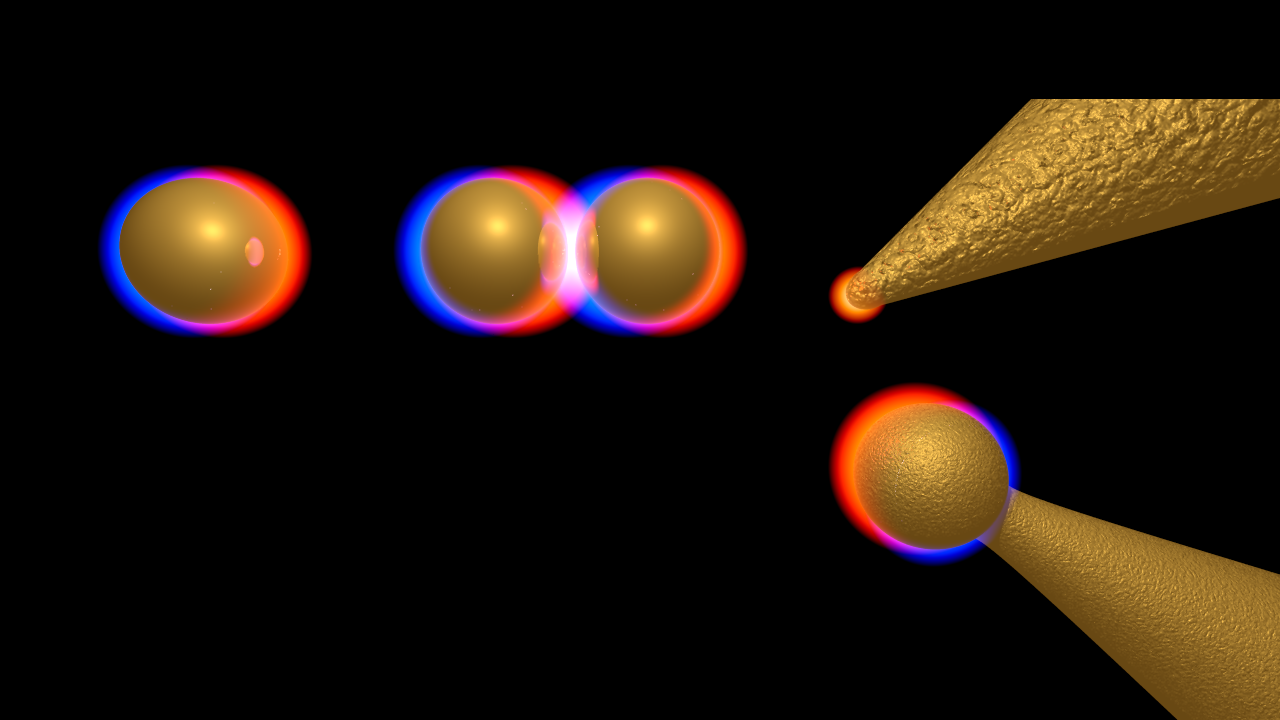
\includegraphics[width=\paperwidth, clip=true, trim=0 0 0 0]{figures/chapter_cover.png}}
}}

\Gls{afm} tips are characterised in a microscope custom-built for optical spectroscopy with simultaneous force and electronic measurements. The microscope is fully automated\footnote{A custom Python application used to control the microscope and all experiments} and capable of running an assortment of experiments, the majority of which have been developed primarily to study the optical response of tips. Its primary function is to take the tips of two opposing AFM probes, align them into a tip-to-tip dimer geometry and demonstrate nm-scale precision spatial control. Using such a setup, the plasmonic behaviour of both individual and coupled tip systems can be investigated. Using spherical AuNP-tipped AFM tips in this way enables dynamical study of a system similar to the prototypical AuNP dimer under various conditions. Significant effort was invested into developing a system with the capabilities to perform these experiments. In this chapter the principles behind it's operation and the design considerations are discussed in depth.

\subimport{./}{mechanical_design}
\subimport{./}{optical_design}
\subimport{./}{electronics_design}
\subimport{./}{afm_design}
\subimport{./}{tip_alignment}

\section{Conclusions}

A custom-built ultra-stable microscope platform, utilising supercontinuum dark-field spectroscopy, low-noise electronics and AFM, is built to accommodate spectral studies of both individual tips and tip dimers. The platform is stable to both temperature and vibration and able to take two tips and align them into a dimer configuration using a modified form of scanning capacitance microscopy. Performance characterisation shows spectral validity between 500--\SI{1100}{nm}, more broadband than standard optical microscopes, with confocal localisation enabling the study of more complex structures than point scatterers. The addition of \si{fA} level current and AFM force measurements results in a system capable of characterising a sub-nm plasmonic dimer system in far more detail than ever before possible.

\ifstandalone
\begin{singlespace}
\printbibliography[notcategory=fullcited]
\end{singlespace}
\fi

\end{document}